\section{Data}
The data used in this study were generated by P. Furth et al. in 2023
\supercite{furth_esr1_2023,furth_overexpression_2023}.

\subsection{Mouse models}
Mouse models allow the study of disease pathophysiology within the context of
physiological endocrine and immunologic function.

\subsection{Samples}
Describe the samples used in the study and how they were collected.
Include the timeline plots from the poster.
Explain the different sequencing steps.

\section{Nextflow and nf-core}
\paragraph{Nextflow} is a workflow management system that enables the
development of reproducible and scalable workflows. It allows the creation of
complex pipelines that can be executed on a variety of platforms, from local
machines to cloud computing environments. Nextflow uses a domain-specific
language (DSL) that simplifies the definition of workflows and enables the reuse
of existing components \supercite{di_tommaso_nextflow_2017}. As a result,
Nextflow has become a popular tool in the bioinformatics community.

\begin{figure}[ht]
    \centering
    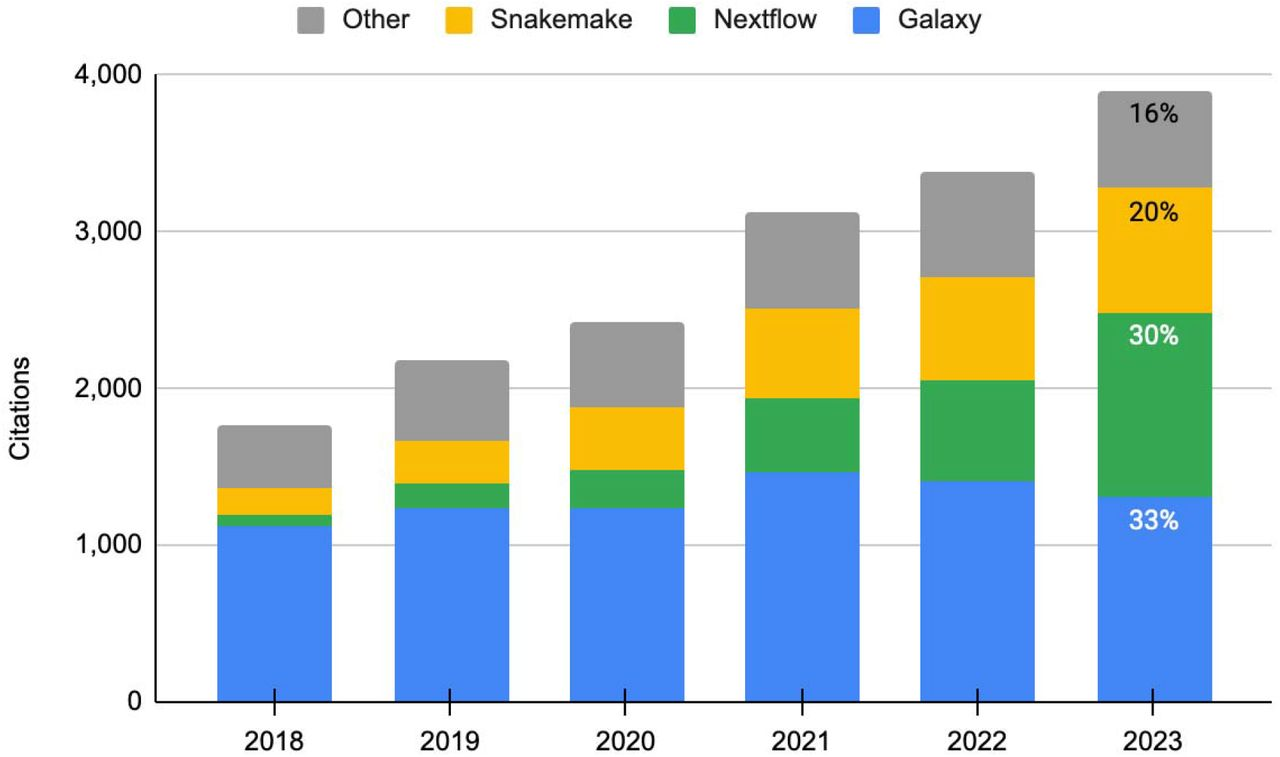
\includegraphics[width=\textwidth]{chapters/materials_and_methods/figures/nextflow_usage.jpg}
    \caption{Workflow management systems} % TODO: Add detailed caption
    \label{fig:nextflow_usage}
\end{figure}

As pointed out by Langer et al. in a recent preprint
\supercite{langer_empowering_2024}, programming-based workflow systems like
Nextflow and Snakemake have gained popularity during the last years, while
GUI-based systems like Galaxy have lost ground. Furthermore, Nextflow has been
the fastest growing workflow system in the last years, with a remarkable 30
percent share of citations in 2023 (\cref{fig:nextflow_usage}). The authors
mostly attribute this to the great quality of the pipelines curated by the
nf-core community \supercite{langer_empowering_2024,grayson_automatic_2023}.

\paragraph{nf-core} is a community-driven project that provides a collection of
high-quality, reproducible, and scalable Nextflow pipelines. These pipelines
cover a wide range of bioinformatics applications, from RNA-seq and ChIP-seq to
single-cell RNA-seq and metagenomics \supercite{ewels_nf-core_2020}. The
community maintains a collection of reusable components, so that developers can
utilize them to speed up the development of new pipelines. The nf-core project
also provides guidelines for best practices in pipeline development, ensuring
that the resulting workflows are robust, efficient, and easy to use
\supercite{ewels_nf-core_2020}.

\section{nf-core/circrna}
The nf-core/circrna pipeline has originally been published by Digby et al. in
2023 \supercite{digby_nf-corecircrna_2023}. Since then, the pipeline has gone
through several updates and improvements. The pipeline can utilize seven
different tools for BSJ detection, including CIRIquant, CIRCexplorer2, circRNA
finder, DCC, find\_circ, MapSplice, and Segemehl. It then annotates the detected
circRNAs using GTF-based and database-based annotation. The pipeline also
extracts the sequences of the circRNAs and quantifies their expression levels
together with the linear transcripts. Finally, the pipeline performs miRNA
interaction analysis using miRanda and TargetScan, and provides several
downstream analyses through a Shiny application. An overview of the pipeline is
shown in \cref{fig:circrna_pipeline}.

\begin{figure}[ht]
    \centering
    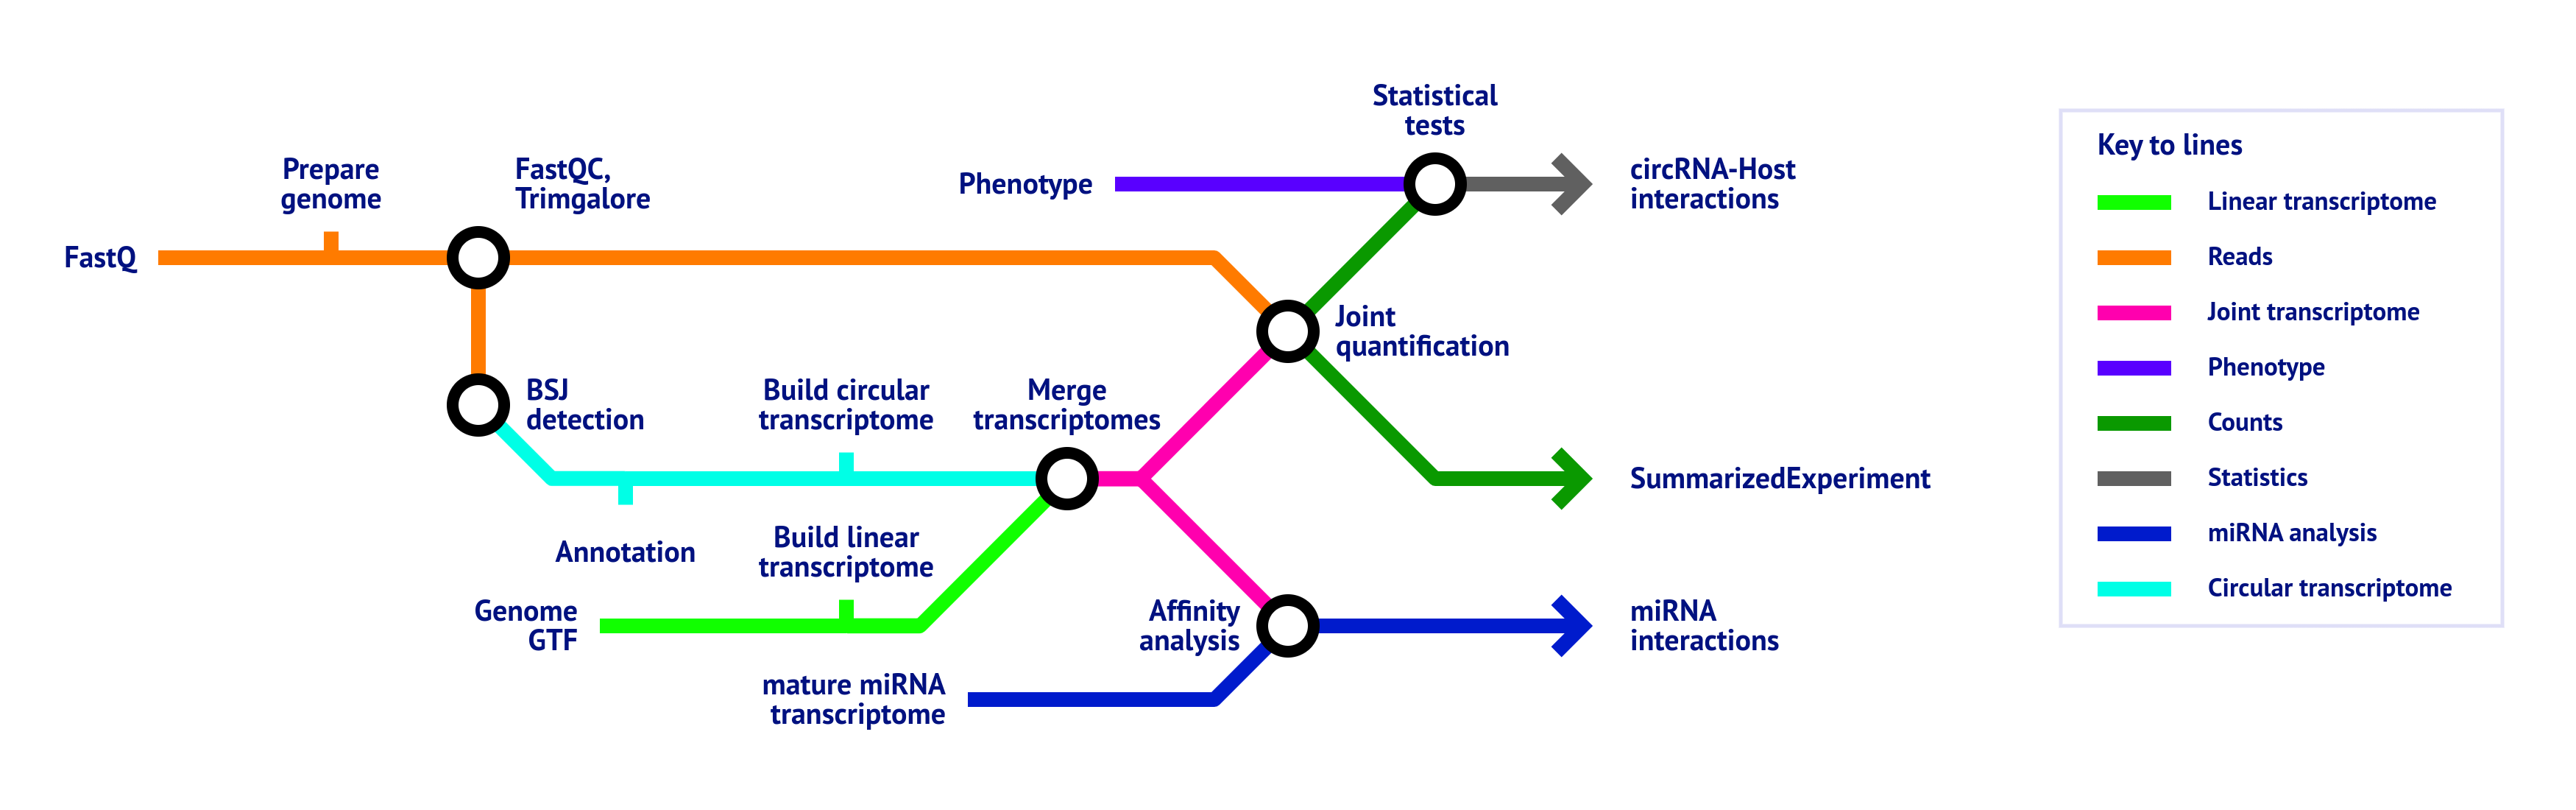
\includegraphics[width=\textwidth]{chapters/materials_and_methods/figures/nf-core_circrna.png}
    \caption{nf-core/circrna} % TODO: Add detailed caption
    \label{fig:circrna_pipeline}
\end{figure}

\subsection{circRNA detection}
What is the main task here?

\subsubsection{CIRI2}
CIRI2 (CircRNA Identifier version 2) is an efficient algorithm designed for de
novo identification of circRNAs. It utilizes a two-step approach: first, it
identifies back-splice junction reads, and then it filters these reads based on
specific criteria to enhance detection accuracy. CIRI2 has been shown to
outperform other tools in terms of sensitivity and specificity, particularly in
datasets with varying sequencing depths\supercite{gao_ciri_2015,zheng_reconstruction_2019}.
This tool is particularly advantageous for large-scale circRNA studies due to
its unbiased nature and ability to handle complex transcriptomes\supercite{chuang_assessing_2023}.

\subsubsection{CIRCexplorer2}
CIRCexplorer2 is another widely used tool that focuses on the detection of
circRNAs by analyzing RNA-seq data. It employs a unique strategy that combines
both back-splice junction reads and linear RNA reads to improve circRNA
identification. CIRCexplorer2 has demonstrated robust performance in various
studies, often ranking high in comparative evaluations against other circRNA
detection tools\supercite{zeng_comprehensive_2017,nicolet_circular_2018}. Its ability to
provide detailed annotations and quantifications of circRNAs makes it a valuable
resource for researchers\supercite{hansen_comparison_2016}.

\subsubsection{circRNA finder}
The circRNA finder is a tool specifically designed for the identification of
circRNAs from RNA-seq data. It employs a read mapping strategy that focuses on
detecting chimeric reads, which are indicative of circRNA formation. This tool
has been effectively utilized in various studies to identify circRNAs across
different biological contexts, although it may have limitations in detecting
circRNAs with non-canonical splice
signals\supercite{sekar_circular_2018,liu_prkra_2022}. Its straightforward
approach makes it accessible for researchers new to
circRNA analysis.

\subsubsection{DCC}
DCC (DCC: Detecting Circular RNAs) is a versatile software that allows for the
detection and quantification of circRNAs from RNA-seq data. It computes
expression levels of circRNAs independently of their linear counterparts, which
is crucial for understanding the functional roles of circRNAs in various
biological processes\supercite{jakobi_profiling_2016,man_profiling_2020}. DCC has been
validated in numerous studies, demonstrating high reliability and accuracy in
circRNA detection\supercite{paraboschi_interpreting_2018}. Its ability to
integrate with other bioinformatics tools further enhances its utility in
comprehensive circRNA analyses.

\subsubsection{find\_circ}
Find\_circ is a widely recognized tool that identifies circRNAs by focusing on
back-splice junctions and employing a filtering strategy based on splice
signals. While it has been effective in many studies, it may not capture
circRNAs with non-canonical splice signals, which can limit its detection
capabilities\supercite{sekar_circular_2018,liu_prkra_2022}. Nonetheless, find\_circ
remains a popular choice for researchers due to its ease of use and integration
with RNA-seq workflows.

\subsubsection{MapSplice}
MapSplice is primarily known for its role in splicing analysis but has also been
adapted for circRNA detection. It utilizes a splice-aware alignment strategy to
identify back-splice junctions, making it suitable for circRNA studies. However,
its performance in circRNA detection may not be as robust as dedicated circRNA
tools like CIRI2 or DCC\supercite{zeng_comprehensive_2017,chuang_nclscan_2016}. MapSplice's
strength lies in its ability to handle complex splicing events, which can be
beneficial in certain research contexts.

\subsubsection{Segemehl}
Segemehl is another tool that has been employed for circRNA detection,
particularly in studies involving complex transcriptomes. It utilizes a unique
alignment strategy that allows for the detection of both linear and circular
transcripts. While Segemehl has shown promise in identifying circRNAs, its
performance can vary depending on the specific dataset and experimental
conditions\supercite{gao_ciri_2015,zeng_comprehensive_2017}. Its flexibility in handling
different types of RNA-seq data makes it a valuable option for researchers
exploring circRNA biology.

\subsection{circRNA annotation}
What is the main task here?

\subsubsection{GTF based annotation}
Describe GTF based annotation

\subsubsection{Database based annotation}
Describe database based annotation

\subsection{circRNA quantification}

Why is this important?

\subsubsection{psirc-quant}
Describe psirc-quant

\subsection{miRNA interaction analysis}
The analysis of circular RNA (circRNA) interactions with microRNAs (miRNAs) is
crucial for understanding the regulatory roles of circRNAs in various biological
processes. Two prominent tools used for predicting circRNA-miRNA interactions
are MiRanda and TargetScan. These tools leverage sequence complementarity and
binding energy calculations to identify potential miRNA binding sites within
circRNA sequences, thereby elucidating their roles as competitive endogenous
RNAs (ceRNAs).

\subsubsection{MiRanda}
MiRanda is a widely utilized algorithm that predicts miRNA targets based on
sequence complementarity and the stability of the RNA duplex formed between the
miRNA and its target. It has been effectively employed in various studies to
analyze circRNA-miRNA interactions. For instance, Vromman et al. noted that
MiRanda is often used alongside TargetScan to predict miRNA binding sites in
circRNA sequences, contributing to a better understanding of circRNA functions
in gene regulation\supercite{vromman_closing_2021}. Similarly, Zhang et al. utilized
MiRanda in conjunction with TargetScan to predict microRNA response elements
(MREs) in differentially expressed circRNAs, demonstrating its utility in
identifying significant interactions\supercite{zhang_microarray_2017}.

\subsubsection{TargetScan}
TargetScan, on the other hand, focuses on the identification of conserved miRNA
binding sites across species, which enhances the reliability of the predicted
interactions. This tool has been integrated into various studies to explore the
regulatory networks involving circRNAs and miRNAs. For example, Jin et al.
employed MiRanda and TargetScan to predict interactions between circRNAs and
miRNAs, reinforcing the hypothesis that circRNAs can act as miRNA
sponges\supercite{jin_changes_2018}. Furthermore, the combination of these tools
allows researchers to construct comprehensive circRNA-miRNA-mRNA networks,
elucidating the complex regulatory mechanisms at play in various
diseases\supercite{he_construction_2021,zhang_construction_2021}.


\subsection{Downstream analyses}
\subsubsection{R-shiny}
\subsubsection{Dimensionality reduction}
\subsubsection{Pathway analysis}
\subsubsection{Differential expression analysis}
\subsubsection{Genome browser}
